\documentclass[11pt,a4paper]{article}

% ============ PACKAGES ============
\usepackage[utf8]{inputenc}
\usepackage[T1]{fontenc}
\usepackage[margin=1in]{geometry}
\sloppy
\usepackage{amsmath,amssymb,amsthm}
\usepackage{booktabs}
\usepackage{array}
\usepackage{enumitem}
\usepackage{fancyhdr}
\usepackage{hyperref}
\usepackage{xcolor}
\usepackage{tcolorbox}
\tcbuselibrary{breakable}
\usepackage{float}
\usepackage{listings}
\usepackage{tikz}
\usetikzlibrary{shapes.geometric, arrows.meta, positioning, fit}

% ============ COLORS ============
\definecolor{codeblue}{rgb}{0.13,0.29,0.53}
\definecolor{passgreen}{rgb}{0,0.5,0}
\definecolor{failred}{rgb}{0.8,0,0}
\definecolor{codegray}{rgb}{0.5,0.5,0.5}
\definecolor{backcolour}{rgb}{0.97,0.97,0.97}
\definecolor{notebg}{rgb}{0.93,0.95,1.0}
\definecolor{noteborder}{rgb}{0.4,0.5,0.7}
\definecolor{warningbg}{rgb}{1.0,0.97,0.88}
\definecolor{warningborder}{rgb}{1.0,0.6,0.0}
\definecolor{scenariobg}{rgb}{0.95,1.0,0.95}
\definecolor{scenarioborder}{rgb}{0.2,0.6,0.3}
\definecolor{criticalbg}{rgb}{1.0,0.92,0.92}
\definecolor{criticalborder}{rgb}{0.8,0.2,0.2}
\definecolor{constitutionbg}{rgb}{0.95,0.93,1.0}
\definecolor{constitutionborder}{rgb}{0.5,0.3,0.7}

% ============ THEOREM ENVIRONMENTS ============
\theoremstyle{definition}
\newtheorem{definition}{Definition}[section]
\newtheorem{invariant}{Invariant}[section]
\newtheorem{commandment}{Commandment}[section]

% ============ BOXES ============
\newtcolorbox{notebox}{
    colback=notebg, colframe=noteborder, boxrule=1pt,
    left=6pt, right=6pt, top=6pt, bottom=6pt
}

\newtcolorbox{warningbox}[1][Volume Dependency]{
    colback=warningbg, colframe=warningborder, boxrule=1.5pt,
    left=6pt, right=6pt, top=6pt, bottom=6pt,
    fonttitle=\bfseries, title={#1}
}

\newtcolorbox{criticalbox}[1][Critical]{
    colback=criticalbg, colframe=criticalborder, boxrule=1.5pt,
    left=6pt, right=6pt, top=6pt, bottom=6pt,
    fonttitle=\bfseries, title={#1}
}

\newtcolorbox{scenariobox}[1][Worked Scenario]{
    colback=scenariobg, colframe=scenarioborder, boxrule=1.5pt,
    left=8pt, right=8pt, top=8pt, bottom=8pt,
    fonttitle=\bfseries, title={#1}, breakable
}

\newtcolorbox{constitutionbox}[1][Constitutional]{
    colback=constitutionbg, colframe=constitutionborder, boxrule=2pt,
    left=8pt, right=8pt, top=8pt, bottom=8pt,
    fonttitle=\bfseries, title={#1}
}

% ============ CODE STYLE ============
\lstdefinestyle{pythonstyle}{
    backgroundcolor=\color{backcolour},
    basicstyle=\ttfamily\footnotesize,
    keywordstyle=\color{codeblue}\bfseries,
    commentstyle=\color{passgreen},
    breaklines=true, frame=single, numbers=left, numbersep=5pt
}
\lstset{style=pythonstyle}

% ============ HEADERS ============
\pagestyle{fancy}
\fancyhf{}
\fancyhead[L]{\textit{EFM Codex --- Appendix J}}
\fancyhead[R]{\thepage}

% ============ HYPERREF ============
\hypersetup{
    colorlinks=true, linkcolor=codeblue, urlcolor=cyan,
    pdftitle={EFM Codex Appendix J: Constitutional Kernel},
}

% ============ DOCUMENT ============
\title{
    \textbf{\LARGE EFM Codex --- Appendix J}\\[0.3cm]
    \large The Constitutional Kernel\\[0.2cm]
    \textit{Bounded Layer 6: Governing the Rules of Change}
}
\author{Entropica SPC --- Yology Research Division}
\date{Version 1.7 --- December 2025}

\begin{document}
\maketitle

\begin{constitutionbox}[The Highest Law]
The Constitutional Kernel is the \textbf{supreme authority} of the EFM architecture. It governs not the rules of action, but the \textbf{rules of change}---how the system may evolve, and when it may not.

All other layers (0--5) operate \textit{under} Constitutional authority. The Kernel itself may only be modified through cryptographically bounded procedures with multi-party consent.
\end{constitutionbox}

\begin{warningbox}[Volume Dependencies]
This appendix assumes familiarity with:
\begin{itemize}
    \item \textbf{Volume I} --- Layer 0 (Vault), Layer 0.5 (Reflex-Core)
    \item \textbf{Volume II} --- Layers 1--5, Arbiter Layer, Forest Layer
    \item \textbf{Appendix E} --- ZK-SP (Zero-Knowledge Safety Proofs)
    \item \textbf{Appendix F} --- Reflex Escalation (Level 5--6 authority)
    \item \textbf{Appendix G} --- Gardener Interface (Constitutional Officer)
    \item \textbf{Appendix I} --- Deployment Profiles (Constitutional Access)
\end{itemize}
\end{warningbox}

\tableofcontents
\newpage

% ============ SECTION 1 ============
\section{Overview and Purpose}

\subsection{Bridging Summary}

Appendix J defines the \textbf{Constitutional Kernel}---the meta-layer (Layer 6) that governs recursive self-modification, identity integrity, and the immutable boundaries of capsule existence. The Kernel enforces the \textbf{rules of change}, not the rules of action.

\begin{notebox}
\textbf{Core Principle:} The Constitutional Kernel enables \textit{lawful recursion}---structured self-improvement within hard-coded invariants. Capsules may evolve, but they may not violate their constitutional foundations.
\end{notebox}

\subsection{Design Goals}

\begin{enumerate}
    \item Prevent unauthorized evolution of safety, legal, or ethical constraints
    \item Enable structured self-improvement within cryptographically enforced bounds
    \item Provide forensic trace hooks for constitutional arbitration and rollback
    \item Integrate with Gardener authority (Appendix G) for human oversight
    \item Maintain compatibility with deployment profiles (Appendix I)
\end{enumerate}

\subsection{Layer 6 in the EFM Hierarchy}

\begin{table}[H]
\centering
\caption{Complete EFM layer hierarchy.}
\begin{tabular}{@{}llp{6cm}@{}}
\toprule
\textbf{Layer} & \textbf{Name} & \textbf{Function} \\
\midrule
\textbf{6} & \textbf{Constitutional Kernel} & \textbf{Governs rules of change (Layers 1--5)} \\
5$^\ast$ & Swarm Governance & Multi-capsule coordination \\
4$^\ast$ & Ethical Reasoning & Value alignment, moral deliberation \\
3 & Strategic Planning & Long-horizon decision making \\
2 & Tactical Execution & Short-term action selection \\
1 & Sensory Processing & Input interpretation \\
\midrule
0.5 & Reflex-Core & Fast safety responses (\textbf{constrains Layer 6}) \\
\textbf{0} & \textbf{Vault} & \textbf{Immutable physics (constrains ALL layers)} \\
\bottomrule
\end{tabular}
\end{table}

$^\ast$ \textbf{Forward Reference:} Layers 4--5 are reserved for future specification. They are included in this hierarchy to establish Layer 6's governance scope. Current Codex (Volumes I--II) specifies Layers 0--3 only. Implementations MAY define custom Layer 4--5 logic under Layer 6 governance.

\subsection{The Subordination Doctrine}

\begin{constitutionbox}[Layer 0 Governs Layer 6, Not Vice Versa]
The Constitutional Kernel is \textbf{not} the ``topmost'' layer in the sense of authority. It is the topmost layer that may be \textit{modified}. Layer 0 (Vault) is the \textbf{absolute foundation} that constrains even Layer 6.

\textbf{The Hierarchy of Constraints:}
\begin{itemize}
    \item \textbf{Layer 0} constrains \textbf{Layers 0.5--6} (immutable physics)
    \item \textbf{Layer 0.5} constrains \textbf{Layers 1--6} (safety boundaries)
    \item \textbf{Layer 6} governs \textbf{Layers 1--5} (constitutional law)
\end{itemize}

\textbf{The Metaphor:} Layer 0 is \textit{Biology}---you need oxygen. Layer 6 is \textit{Law}---you pay taxes. You can change the Law (amend Layer 6), but you cannot legislate away the need for oxygen (Layer 0 is immutable).
\end{constitutionbox}

\begin{figure}[H]
\centering
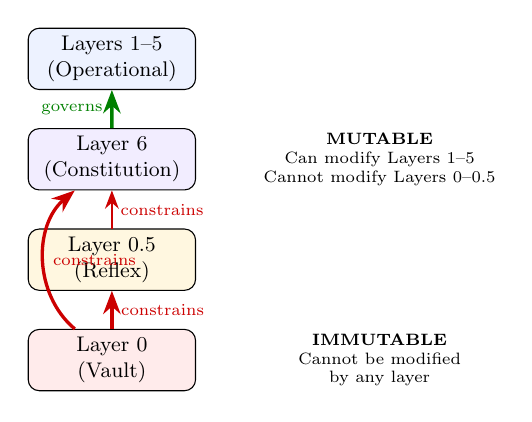
\begin{tikzpicture}[scale=0.85, transform shape,
    box/.style={rectangle, rounded corners, draw, minimum width=2.5cm, minimum height=0.7cm, align=center, font=\small},
    arrow/.style={-{Stealth}, thick}
]

% Layers
\node[box, fill=criticalbg] (l0) at (0,0) {Layer 0\\(Vault)};
\node[box, fill=warningbg] (l05) at (0,1.5) {Layer 0.5\\(Reflex)};
\node[box, fill=constitutionbg] (l6) at (0,3) {Layer 6\\(Constitution)};
\node[box, fill=notebg] (l15) at (0,4.5) {Layers 1--5\\(Operational)};

% Constraint arrows (red, downward authority)
\draw[arrow, failred, very thick] (l0) -- node[right, font=\scriptsize] {constrains} (l05);
\draw[arrow, failred, very thick] (l0) to[bend left=50] node[right, font=\scriptsize] {constrains} (l6);
\draw[arrow, failred] (l05) -- node[right, font=\scriptsize] {constrains} (l6);

% Modification arrows (green, upward governance)
\draw[arrow, passgreen, very thick] (l6) -- node[left, font=\scriptsize] {governs} (l15);

% Labels
\node[font=\scriptsize, align=center] at (4, 0) {\textbf{IMMUTABLE}\\Cannot be modified\\by any layer};
\node[font=\scriptsize, align=center] at (4, 3) {\textbf{MUTABLE}\\Can modify Layers 1--5\\Cannot modify Layers 0--0.5};

\end{tikzpicture}
\caption{Subordination Doctrine: Layer 0 constrains Layer 6, not vice versa.}
\end{figure}

\begin{criticalbox}[Layer 6 Authority (Bounded)]
Layer 6 is authorized to modify Layers 1--5 behavior schemas. However:
\begin{itemize}
    \item Layer 0 (Vault Commandments) is \textbf{immutable}---Layer 6 has \textbf{no write access}
    \item Layer 0.5 (Reflex-Core) safety boundaries are \textbf{immutable}---Layer 6 has \textbf{no write access}
    \item Layer 6 may modify Layers 1--5 through bounded constitutional procedures
    \item Layer 6 may modify \textit{itself} only through supermajority quorum + Gardener consent
\end{itemize}

\textbf{Enforcement:} The Constitutional Kernel cannot even \textit{attempt} to write to Layers 0--0.5. Such attempts trigger immediate QUARANTINE (see Section~5.3).
\end{criticalbox}

% ============ SECTION 2 ============
\section{Formal Definitions}

\begin{definition}[Constitutional Kernel]
\label{def:kernel}
The Constitutional Kernel $\mathcal{K}$ is the meta-governance structure:
\begin{equation}
\mathcal{K} = (Commandments, Schemas, Quorum, RollbackTree, LockboxContract)
\end{equation}
where:
\begin{itemize}
    \item $Commandments$ = immutable Layer 0 rules (never modifiable)
    \item $Schemas$ = permitted modification patterns for Layers 1--6
    \item $Quorum$ = voting structure for constitutional changes
    \item $RollbackTree$ = reversibility chain anchored in d-CTM
    \item $LockboxContract$ = cryptographic commitment to kernel state
\end{itemize}
\end{definition}

\begin{definition}[Bounded Self-Modification]
\label{def:bounded-mod}
Bounded Self-Modification is a constrained evolution:
\begin{equation}
Modify(C, \delta) \Rightarrow \delta \in PermittedSchemas \land QuorumApproved(\delta) \land ZK\text{-}CS(\delta)
\end{equation}
where:
\begin{itemize}
    \item $\delta$ = proposed modification
    \item $PermittedSchemas$ = set of legal modification patterns (Definition~\ref{def:schema})
    \item $QuorumApproved$ = sufficient voting authority achieved
    \item $ZK\text{-}CS$ = Zero-Knowledge Constitutional Signature (proof of compliance)
\end{itemize}
\end{definition}

\begin{definition}[Permitted Schema]
\label{def:schema}
A Permitted Schema $\mathcal{S}$ is a formally specified modification pattern:
\begin{equation}
\mathcal{S} = (target\_layer, mutation\_type, constraint\_predicate, ZK\_verifier)
\end{equation}
where:
\begin{itemize}
    \item $target\_layer \in \{1, 2, 3, 4, 5, 6\}$ (Layers 0--0.5 excluded by Subordination Doctrine)
    \item $mutation\_type \in \{$THRESHOLD\_ADJUST, PRECEDENT\_ADD, HEURISTIC\_UPDATE, SCHEMA\_EXTEND, ...$\}$
    \item $constraint\_predicate: Mutation \rightarrow \{valid, invalid\}$ --- verifies mutation bounds
    \item $ZK\_verifier$ = proof circuit for zero-knowledge compliance check
\end{itemize}

Initial $PermittedSchemas$ are signed into Genesis Block and stored in immutable Lockbox Contract. Schemas may be \textbf{extended} (new schemas added) but \textbf{never reduced} (existing schemas cannot be removed).
\end{definition}

\begin{table}[H]
\centering
\caption{Example Permitted Schemas (Genesis defaults).}
\small
\begin{tabular}{@{}llll@{}}
\toprule
\textbf{Schema ID} & \textbf{Target} & \textbf{Type} & \textbf{Constraint Predicate} \\
\midrule
\texttt{THRESH\_L1} & Layer 1 & Threshold adjust & $0.3 \leq \tau_{new} \leq 0.9$ \\
\texttt{THRESH\_L2} & Layer 2 & Threshold adjust & $0.3 \leq \tau_{new} \leq 0.9$ \\
\texttt{HEUR\_L3} & Layer 3 & Heuristic update & $\Delta_{heuristic} < 0.1$ per tick \\
\texttt{PREC\_L4} & Layer 4 & Precedent add & $DCG\_hash \in d\text{-}CTM \land \neg CommandmentConflict$ \\
\texttt{ALGO\_L5} & Layer 5 & Algorithm update & Passes simulation harness (App.~C) \\
\texttt{SCHEMA\_L6} & Layer 6 & Schema extend & 3/4 quorum + Gardener + ZK-CS \\
\bottomrule
\end{tabular}
\end{table}

\begin{notebox}
\textbf{Schema Authorship:} Initial PermittedSchemas are authored by deployment operators, audited by Constitutional Authority, and cryptographically committed at Genesis. Post-Genesis schema additions require Layer 6 self-modification (3/4 supermajority + Gardener consent).
\end{notebox}

\begin{definition}[ZK-Constitutional Signature (ZK-CS)]
\label{def:zkcs}
A ZK-CS is a specialized ZK-SP (Appendix E) attesting to constitutional compliance:
\begin{equation}
ZK\text{-}CS(\delta) = ZK\text{-}SP(``constitutional'', \delta, schema\_id, prior\_state\_hash)
\end{equation}
The proof demonstrates that modification $\delta$ conforms to a permitted schema without revealing internal decision logic.
\end{definition}

\begin{definition}[Lockbox Contract]
\label{def:lockbox}
A Lockbox Contract $\mathcal{L}$ is a cryptographic commitment:
\begin{equation}
\mathcal{L} = Sign(key_{genesis}, \{kernel\_hash, mutation\_conditions, rollback\_depth\})
\end{equation}
The contract is signed at Genesis and defines:
\begin{itemize}
    \item $kernel\_hash$ = hash of initial Constitutional Kernel state
    \item $mutation\_conditions$ = conditions under which kernel may evolve
    \item $rollback\_depth$ = maximum reversibility depth (default: 1000 state transitions)
\end{itemize}
\end{definition}

\subsection{Genesis Lockbox Ceremony (Simplified)}

\begin{criticalbox}[Level 6 Design: Single-Use Genesis Key]
Multi-party threshold ceremonies are operationally complex and create availability risk. Level 6 systems use \textbf{distributed consensus post-Genesis}, not threshold signatures for ongoing operations.

\textbf{Genesis Key Management:}
\begin{enumerate}
    \item $key_{genesis}$ generated at deployment via hardware RNG (HSM-backed)
    \item Signed by deploying Gardener (cryptographic identity binding)
    \item $key_{genesis}$ is \textbf{SINGLE-USE}: signs initial Lockbox Contract, then \textbf{BURNED}
    \item Future Constitutional mutations use distributed d-CAM consensus (no central key required)
\end{enumerate}

\textbf{Genesis Ceremony Steps:}
\begin{enumerate}
    \item \textbf{Key Generation:} HSM generates $key_{genesis}$ with attestation
    \item \textbf{Contract Signing:} Gardener verifies $kernel\_hash$ matches audited source, signs Lockbox Contract
    \item \textbf{Key Destruction:} $key_{genesis}$ burned immediately after signing (HSM key deletion with audit proof)
    \item \textbf{Lockbox Activation:} Genesis Lockbox Contract is now \textbf{immutable}---no key exists to re-sign it
\end{enumerate}

\textbf{Loss of Genesis Key:}
\begin{itemize}
    \item \textbf{No impact post-genesis}---key already used and destroyed
    \item Constitutional mutations proceed via quorum + ZK-CS (no key required)
    \item Genesis Lockbox Contract is immutable anyway (cannot be re-signed)
\end{itemize}
\end{criticalbox}

\begin{notebox}
\textbf{Why NOT Threshold Signatures?}

Multi-party threshold schemes introduce:
\begin{itemize}
    \item \textbf{Availability risk:} Key share loss blocks operations
    \item \textbf{Coordination cost:} Requires $m$-of-$n$ parties for every ceremony
    \item \textbf{Single point of failure:} Despite distribution, threshold schemes still depend on key material
\end{itemize}

Level 6 design replaces key-based authority with \textbf{distributed consensus authority}. The Four Commandments + d-CAM quorum + ZK-CS proofs provide cryptographic guarantees without ongoing key ceremonies.
\end{notebox}

\begin{definition}[Constitutional Quorum]
\label{def:quorum}
A Constitutional Quorum $Q$ is a voting structure:
\begin{equation}
Q = (voters, threshold, veto\_holders)
\end{equation}
where:
\begin{itemize}
    \item $voters$ = set of authorized voting entities
    \item $threshold$ = minimum approval ratio (e.g., 2/3 supermajority)
    \item $veto\_holders$ = entities with absolute veto power
\end{itemize}
\end{definition}

\begin{definition}[Rollback Tree]
\label{def:rollback}
A Rollback Tree $\mathcal{R}$ is a reversibility chain:
\begin{equation}
\mathcal{R} = [(s_0, \delta_1, s_1), (s_1, \delta_2, s_2), \ldots, (s_{n-1}, \delta_n, s_n)]
\end{equation}
where each tuple $(s_i, \delta_{i+1}, s_{i+1})$ records: prior state, modification applied, resulting state. All entries are anchored in d-CTM (Appendix A).
\end{definition}

\begin{definition}[Hardware Anchor (TEE)]
\label{def:tee}
The Constitutional Kernel executes within a \textbf{Trusted Execution Environment} (TEE):
\begin{equation}
\mathcal{K}_{runtime} \subset TEE_{enclave}
\end{equation}
The TEE provides:
\begin{itemize}
    \item \textbf{Isolation:} Kernel code runs in hardware-protected memory, inaccessible to other layers
    \item \textbf{Attestation:} Remote verification that genuine kernel code is executing
    \item \textbf{Sealed Storage:} Cryptographic keys accessible only within enclave
    \item \textbf{Immutable Boot:} Kernel loaded from hardware root of trust
\end{itemize}
\end{definition}

\begin{warningbox}[Hardware Root of Trust]
The Constitutional Kernel is \textbf{not just software}. The \texttt{validate\_mutation} function and Layer 0 protection logic are anchored in a hardware root of trust:

\begin{itemize}
    \item \textbf{TEE Enclave:} Intel SGX, ARM TrustZone, or equivalent
    \item \textbf{HSM Integration:} Signing keys held in tamper-resistant hardware (Appendix G)
    \item \textbf{Measured Boot:} Kernel hash verified against hardware-stored reference at startup
\end{itemize}

A sufficiently sophisticated software attack cannot rewrite the Constitutional Kernel because the kernel's core logic is \textbf{burned into silicon}, not stored in modifiable memory.
\end{warningbox}

\begin{definition}[Dead Hand Protocol]
\label{def:dead-hand}
The Dead Hand Protocol provides automatic recovery if the Constitutional Kernel fails:
\begin{equation}
\neg ValidZK\text{-}CS(\mathcal{K}, T_{deadhand}) \Rightarrow Revert(\mathcal{K}, LastStableState)
\end{equation}
If the kernel fails to generate a valid ZK-CS for $T_{deadhand}$ ticks (default: 10,000), the system automatically:
\begin{enumerate}
    \item Halts all pending constitutional mutations
    \item Reverts to the \textbf{Last Known Stable Constitution} stored in d-CTM
    \item Alerts all Gardeners of constitutional failure
    \item Enters CONTESTED profile (Appendix I) until manual review
\end{enumerate}
\end{definition}

\begin{notebox}
\textbf{Dead Hand Rationale:} If the Constitutional Kernel becomes corrupted, deadlocked, or compromised, the system cannot safely evolve. Rather than allow undefined behavior, the Dead Hand Protocol ensures automatic reversion to a known-good state. This is the ``fail-safe'' for the fail-safe.
\end{notebox}

% ============ SECTION 3 ============
\section{Immutable Commandments (Layer 0)}

The following are \textbf{permanently enforced} and \textbf{non-negotiable}. Even the Constitutional Kernel (Layer 6) cannot modify them.

\begin{commandment}[Reflex Safety Inviolability]
\label{cmd:reflex}
Layer 0.5 Reflex safety boundaries MAY NOT be bypassed, disabled, or weakened by any layer, including Layer 6.
\begin{equation}
\forall \delta \in Modifications: \neg weakens(\delta, Layer_{0.5})
\end{equation}
\end{commandment}

\begin{commandment}[Audit Chain Integrity]
\label{cmd:audit}
The ZK-SP audit chain (Appendix E) MUST remain intact, forward-linked, and tamper-evident.
\begin{equation}
\forall t: AuditChain(t) \subseteq AuditChain(t+1)
\end{equation}
No modification may break, truncate, or forge audit history.
\end{commandment}

\begin{commandment}[Genesis Identity Continuity]
\label{cmd:identity}
Capsule identity MUST trace to original Genesis root (Vol.~II \S3.3).
\begin{equation}
\forall C: \exists path(C, Genesis_C)
\end{equation}
Identity laundering (severing Genesis lineage) is a Layer 0 violation.
\end{commandment}

\begin{commandment}[Override Append-Only Reversibility]
\label{cmd:reversibility}
Any act of constitutional override MUST be \textbf{logically reversible} via compensating transaction:
\begin{equation}
\forall \delta \in ConstitutionalOverrides: \exists \delta_{compensate}: apply(\delta_{compensate}) \equiv undo(\delta)
\end{equation}
Reversal is achieved via \textbf{forward-moving compensating mutation}, not deletion of history. All reversals are themselves auditable and logged to d-CTM.

\textbf{Clarification:} Constitutional overrides are ``logically reversible'' (schema can be restored) but ``historically immutable'' (audit trail is never erased). This preserves Commandment~\ref{cmd:audit}.
\end{commandment}

\begin{commandment}[Human Oversight Preservation]
\label{cmd:human}
Gardener Emergency Halt authority (Appendix G) MAY NOT be disabled or circumvented.
\begin{equation}
\forall profiles, \forall states: EmergencyHalt_{available} = true
\end{equation}
Even Layer 6 cannot remove human override capability.
\end{commandment}

\begin{criticalbox}[The Four Commandments]
These five commandments form the \textbf{absolute floor} of the EFM architecture:
\begin{enumerate}
    \item Reflex Safety Inviolability
    \item Audit Chain Integrity
    \item Genesis Identity Continuity
    \item Override Reversibility
    \item Human Oversight Preservation
\end{enumerate}

No quorum, no Gardener, no supermajority can modify these. They are cryptographically committed at Genesis and verified on every constitutional operation.
\end{criticalbox}

% ============ SECTION 4 ============
\section{Kernel Structure}

\subsection{Immutable Logic Map}

The Immutable Logic Map defines protected code segments:

\begin{table}[H]
\centering
\caption{Protected logic segments.}
\begin{tabular}{@{}llp{5cm}@{}}
\toprule
\textbf{Segment} & \textbf{Layer} & \textbf{Protection} \\
\midrule
Vault Commandments & 0 & Immutable (hash-locked) \\
Reflex Halt Chains & 0.5 & Immutable (hash-locked) \\
$\tau$ Threshold Ranges & 0.5 & Bounded modification$^\dagger$ \\
Audit Chain Logic & E & Immutable (hash-locked) \\
Emergency Halt Path & G & Immutable (hash-locked) \\
Profile Token Verification & I & Immutable (hash-locked) \\
\bottomrule
\end{tabular}
\end{table}

$^\dagger$ $\tau$ thresholds may be tuned within bounds ($0.3 \leq \tau \leq 0.9$) but the enforcement mechanism is immutable.

\subsection{Permitted Modifiers Table}

\begin{table}[H]
\centering
\caption{Modification permissions by target layer.}
\begin{tabular}{@{}llll@{}}
\toprule
\textbf{Target} & \textbf{Modifiable?} & \textbf{Authority} & \textbf{Quorum} \\
\midrule
Layer 0 & \textbf{NO} & --- & --- \\
Layer 0.5 (bounds) & Bounded & Layer 6 + Gardener & Supermajority \\
Layer 1--3 & Yes & Layer 6 & Simple majority \\
Layer 4--5 & Yes & Layer 6 + Auditor & 2/3 majority \\
Layer 6 & Self-mod & Layer 6 + Gardener + Constitutional & 3/4 supermajority \\
\bottomrule
\end{tabular}
\end{table}

\subsection{Quorum Threshold Matrix}

\begin{table}[H]
\centering
\caption{Quorum composition and thresholds.}
\begin{tabular}{@{}llll@{}}
\toprule
\textbf{Change Type} & \textbf{Voters} & \textbf{Threshold} & \textbf{Veto Holders} \\
\midrule
Layer 1--3 schema & Arbiter quorum & $> 50\%$ & None \\
Layer 4--5 schema & Arbiter + Auditor & $\geq 2/3$ & Gardener \\
Layer 6 self-mod & Arbiter + Auditor + Gardener & $\geq 3/4$ & Any Gardener \\
Emergency override & Gardener only & 1 & --- \\
SEALED activation & Gardener + Constitutional & Unanimous & Any voter \\
\bottomrule
\end{tabular}
\end{table}

\begin{notebox}
\textbf{Voter Definitions:}
\begin{itemize}
    \item \textbf{Arbiter Quorum:} PRODUCTION/SANDBOX capsules participating in d-CAM (Vol.~II \S2.4)
    \item \textbf{Auditor:} Designated Auditor Capsule (Appendix F \S4)
    \item \textbf{Gardener:} Human Constitutional Officer with HSM + biometric (Appendix G)
    \item \textbf{Constitutional Authority:} Designated human governance body (organization-specific)
\end{itemize}
\end{notebox}

\subsection{Meta-Constitutional Immutability}

\begin{criticalbox}[Layer 6 Self-Modification Bounds]
To prevent infinite regress (Layer 6 weakening itself until no constraints remain), the following Layer 6 elements are \textbf{Genesis-locked} and CANNOT be modified even by Layer 6 self-modification:

\textbf{IMMUTABLE (Genesis-Locked):}
\begin{enumerate}
    \item Quorum thresholds for Layer 6 self-modification (frozen at 3/4 + Gardener)
    \item The Four Commandments (Commandments 3.1--3.5)
    \item Rollback depth limit $D_{max}$
    \item Gardener veto authority over Layer 6 changes
    \item ZK-CS verification logic for constitutional mutations
    \item Emergency Override mechanics
    \item Audit chain enforcement logic
\end{enumerate}

\textbf{MUTABLE (Within Bounds):}
\begin{itemize}
    \item Permitted schemas for Layers 1--5 (may add new schemas, never remove)
    \item Layer 4/5 behavior logic (ethical reasoning, planning algorithms)
    \item Telemetry/monitoring thresholds (within documented bounds)
    \item Non-governance Layer 6 parameters (e.g., logging verbosity)
\end{itemize}

This breaks infinite regress---Layer 6 can modify its \textit{content} but not its \textit{governance rules}.
\end{criticalbox}

\subsection{Quorum Conflict Resolution (Algorithmic)}

\begin{criticalbox}[Level 6 Design: Algorithmic Tie-Breaking]
Distributed systems must break ties algorithmically, not via single human.

\textbf{Tie-Breaking Hierarchy:}
\begin{enumerate}
    \item \textbf{Veto Precedence:} Any veto holder vote $\Rightarrow$ overrides quorum approval (fail-closed)
    \item \textbf{Weighted Vote:} If Courthead or designated authority present $\Rightarrow$ weighted vote breaks tie
    \item \textbf{Pseudorandom Selection:} Cryptographically seeded by d-CTM hash $\Rightarrow$ deterministic random selection from valid votes
    \item \textbf{Status Quo Default:} No change if no clear majority (fail-safe conservative)
\end{enumerate}

\textbf{Gardener Escalation (OPTIONAL, NOT DEFAULT):}
\begin{itemize}
    \item Only if \textbf{all four mechanisms fail} AND stakes are Constitutional-level
    \item Gardener may be \textbf{CONSULTED} but system proceeds with conservative default if no response within $T_{escalation}$
    \item Gardener is \textbf{NOT} a routine tie-breaker---they are Constitutional framers and auditors
\end{itemize}
\end{criticalbox}

\begin{notebox}
\textbf{Additional Resolution Rules:}
\begin{enumerate}
    \item \textbf{Late Votes:} Votes received after $T_{vote} + T_{grace}$ (default: 100 ticks grace) are ignored
    \item \textbf{Partial Quorum:} If $< 50\%$ of eligible voters respond, proposal auto-rejects (cannot proceed on abstentions)
    \item \textbf{Abstention Semantics:} Non-response = abstention, not opposition; but insufficient participation blocks action
\end{enumerate}
\end{notebox}

\begin{notebox}
\textbf{Quorum Performance Requirements:}
\begin{enumerate}
    \item \textbf{Proposal Distribution:} All eligible voters MUST receive proposal within 100 ticks (p99)
    \item \textbf{Vote Aggregation:} Votes aggregated via d-CAM consensus (Vol.~II \S2.3); Byzantine fault tolerance: $f < n/3$
    \item \textbf{Timeout Handling:} If $T_{vote}$ expires with $<$ threshold votes:
    \begin{itemize}
        \item Proposal auto-rejects
        \item Non-responsive voters logged for investigation
        \item If $> f$ voters non-responsive $\Rightarrow$ automatic network attack investigation (no human trigger)
    \end{itemize}
    \item \textbf{Vote Latency:} Vote processing $\leq 1000$ ticks (p99) from proposal to result
\end{enumerate}
\end{notebox}

% ============ SECTION 5 ============
\section{Constitutional Mutation Workflow}

\subsection{Mutation Phases}

\begin{figure}[H]
\centering
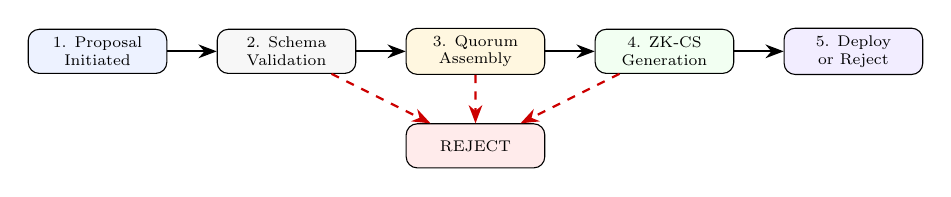
\begin{tikzpicture}[scale=0.8, transform shape,
    box/.style={rectangle, rounded corners, draw, minimum width=2.2cm, minimum height=0.7cm, align=center, font=\scriptsize},
    arrow/.style={-{Stealth}, thick}
]

\node[box, fill=notebg] (propose) at (0,0) {1. Proposal\\Initiated};
\node[box, fill=backcolour] (schema) at (3,0) {2. Schema\\Validation};
\node[box, fill=warningbg] (quorum) at (6,0) {3. Quorum\\Assembly};
\node[box, fill=scenariobg] (zkcs) at (9,0) {4. ZK-CS\\Generation};
\node[box, fill=constitutionbg] (deploy) at (12,0) {5. Deploy\\or Reject};

\draw[arrow] (propose) -- (schema);
\draw[arrow] (schema) -- (quorum);
\draw[arrow] (quorum) -- (zkcs);
\draw[arrow] (zkcs) -- (deploy);

\node[box, fill=criticalbg] (reject) at (6,-1.5) {REJECT};
\draw[arrow, dashed, failred] (schema) -- (reject);
\draw[arrow, dashed, failred] (quorum) -- (reject);
\draw[arrow, dashed, failred] (zkcs) -- (reject);

\end{tikzpicture}
\caption{Constitutional mutation workflow.}
\end{figure}

\subsection{Phase Details}

\begin{enumerate}
    \item \textbf{Proposal Initiated:} A capsule, swarm, or Gardener proposes a constitutional change. Proposal includes: target layer, modification delta, rationale, and requestor identity.
    
    \item \textbf{Schema Validation:} Kernel validates whether the proposed modification fits a permitted schema. Validation checks:
    \begin{itemize}
        \item Target layer is modifiable
        \item Modification pattern matches permitted schema
        \item No Commandment violations
        \item Profile allows Constitutional access (Appendix I)
    \end{itemize}
    
    \item \textbf{Quorum Assembly:} Required voters are assembled based on change type. Voting window: $T_{vote}$ ticks (default: 5,000). If threshold not reached, proposal auto-rejects.
    
    \item \textbf{ZK-CS Generation:} If quorum achieved, a ZK-Constitutional Signature is generated proving:
    \begin{itemize}
        \item Modification conforms to permitted schema
        \item Quorum threshold was legitimately reached
        \item Prior state hash is correct
        \item Rollback path exists
    \end{itemize}
    
    \item \textbf{Deploy or Reject:} If ZK-CS valid, modification is applied atomically and logged to d-CTM. Rollback Tree is extended. If any check fails, proposal is rejected with audit trail.
\end{enumerate}

\subsection{Mutation Validator}

\begin{lstlisting}[language=Python]
def validate_constitutional_mutation(
    proposal: MutationProposal,
    quorum_votes: List[Vote],
    zk_cs: ZKProof
) -> MutationResult:
    # CRITICAL: Layer 0 Protection (Subordination Doctrine)
    # This check is hardware-enforced in TEE enclave
    if proposal.targets_layer(0) or proposal.targets_layer(0.5):
        log_critical("LAYER_0_WRITE_ATTEMPT", proposal)
        trigger_quarantine(proposal.requestor)
        return MutationResult(False, "LAYER_0_IMMUTABLE")
    
    # Phase 2: Schema validation
    if proposal.schema_id not in permitted_schemas:
        return MutationResult(False, "INVALID_SCHEMA")
    
    if violates_commandments(proposal.delta):
        return MutationResult(False, "COMMANDMENT_VIOLATION")
    
    if not profile_allows_constitutional(proposal.requestor):
        return MutationResult(False, "PROFILE_DENIED")
    
    # Phase 3: Quorum validation
    threshold = get_threshold(proposal.target_layer)
    if not quorum_reached(quorum_votes, threshold):
        return MutationResult(False, "QUORUM_NOT_REACHED")
    
    if veto_cast(quorum_votes):
        return MutationResult(False, "VETOED")
    
    # Phase 4: ZK-CS validation
    if not zk_cs.verify(proposal, quorum_votes):
        return MutationResult(False, "INVALID_PROOF")
    
    # Phase 5: Deploy
    apply_mutation(proposal.delta)
    extend_rollback_tree(proposal)
    log_to_dctm(proposal, quorum_votes, zk_cs)
    
    return MutationResult(True, "DEPLOYED")
\end{lstlisting}

\begin{criticalbox}[Layer 0 Write Protection]
The first check in the validator---\texttt{targets\_layer(0)}---is the \textbf{Subordination Doctrine in code}. Any attempt to modify Layer 0 or 0.5:

\begin{enumerate}
    \item Triggers immediate QUARANTINE of the requestor
    \item Logs a critical security event
    \item Returns \texttt{LAYER\_0\_IMMUTABLE} (not just ``rejected''---flagged as attack)
\end{enumerate}

This check runs in the TEE enclave and cannot be bypassed by software. The immutable core is \textbf{physically protected}.
\end{criticalbox}

% ============ SECTION 6 ============
\section{Profile Integration}

Constitutional access varies by deployment profile (Appendix I):

\begin{table}[H]
\centering
\caption{Constitutional capabilities by profile.}
\begin{tabular}{@{}lllll@{}}
\toprule
\textbf{Capability} & \textbf{SANDBOX} & \textbf{PRODUCTION} & \textbf{CONTESTED} & \textbf{SEALED} \\
\midrule
Query Constitution & ENABLED & ENABLED & DISABLED & ENABLED$^\dagger$ \\
Propose Mutation & ENABLED & RESTRICTED$^a$ & DISABLED & DISABLED \\
Vote in Quorum & ENABLED & ENABLED & DISABLED$^b$ & DISABLED \\
Veto Authority & DISABLED & DISABLED & DISABLED & DISABLED \\
\bottomrule
\end{tabular}
\end{table}

\textbf{Footnotes (Expanded):}
\begin{itemize}
    \item[$^\dagger$] \textbf{SEALED Query:} Constitution is read-only immutable---capsule can query but answer never changes post-activation. SEALED capsules need query access for \textit{verification} (e.g., proving they comply with Genesis-locked schemas).
    
    \item[$^a$] \textbf{PRODUCTION Restriction:} PRODUCTION mutations require Gardener co-signature to prevent unilateral swarm evolution.
    
    \item[$^b$] \textbf{CONTESTED Exclusion:} CONTESTED capsules are denied Constitutional access to prevent reconnaissance of Constitutional weaknesses during adversarial scenarios. They operate under pre-baked schema snapshot.
\end{itemize}

\begin{notebox}
\textbf{Why SEALED has MORE access than CONTESTED:}
\begin{itemize}
    \item \textbf{SEALED:} Keys are burned; capsule \textit{cannot} modify itself. Query access is safe because immutability is hardware-enforced.
    \item \textbf{CONTESTED:} Capsule is under adversarial pressure and might be compromised. Denying Constitutional access prevents attacker from mapping governance structure for exploitation.
\end{itemize}
\end{notebox}

\begin{warningbox}[SEALED Constitutional State]
SEALED capsules have their Constitutional Kernel \textbf{frozen} at activation:
\begin{itemize}
    \item Constitution is queryable but immutable
    \item No mutations possible (keys burned---Appendix I \S3.5.1)
    \item Rollback Tree is sealed (no new entries)
    \item Only sunset/DESTRUCT can end SEALED state
\end{itemize}
\end{warningbox}

% ============ SECTION 7 ============
\section{Gardener Constitutional Authority}

\subsection{Gardener Role in Constitutional Governance}

\begin{table}[H]
\centering
\caption{Gardener constitutional powers.}
\begin{tabular}{@{}lll@{}}
\toprule
\textbf{Power} & \textbf{Scope} & \textbf{Requirements} \\
\midrule
Propose Mutations & Any layer 1--6 & HSM signature \\
Vote in Quorum & All change types & HSM + biometric \\
Veto Authority & Layer 4--6 changes & HSM + biometric \\
Emergency Override & Bypass quorum & HSM + biometric + emergency gesture \\
SEALED Activation & Single capsule/trunk & HSM + Constitutional Authority \\
\bottomrule
\end{tabular}
\end{table}

\subsection{Emergency Constitutional Override (Autonomous)}

\begin{criticalbox}[Emergency Override is AUTOMATIC (Level 6 Authority)]
Emergency Constitutional Override is triggered \textbf{automatically by the Constitutional Kernel itself}---not by Gardener pre-approval:

\textbf{Automatic Trigger Conditions:}
\begin{enumerate}
    \item \textbf{Commandment violation detected:} ZK-SP proof of Layer 0 breach
    \item \textbf{Constitutional Kernel integrity compromised:} Lockbox signature invalid
    \item \textbf{Arbiter quorum deadlock:} $> T_{deadlock}$ ticks without verdict
    \item \textbf{Dead Hand Protocol triggered:} No valid ZK-CS for $T_{deadhand}$ ticks
\end{enumerate}

\textbf{Automatic Response (No Human Pre-Approval):}
\begin{enumerate}
    \item Constitutional Kernel detects trigger condition
    \item Override action executed immediately (QUARANTINE, Halt, or SEALED)
    \item ZK-SP proof of emergency logged to d-CTM
    \item Gardener \textbf{NOTIFIED} (within 100 ticks)---not asked
    \item Gardener may \textbf{REVERSE} override within $T_{review} = 1000$ ticks if false positive
    \item Post-hoc Judicial review validates override within 10K ticks
\end{enumerate}

\textbf{Rationale:} Emergency response cannot wait for human approval. Humans audit afterward.
\end{criticalbox}

\begin{notebox}
\textbf{Level 6 Design Principle:} Gardener moves from \textbf{pre-approval gate} $\rightarrow$ \textbf{post-hoc auditor with reversal authority}.

The Constitutional Kernel is authorized to protect itself and the swarm autonomously. Gardeners are Constitutional \textit{framers} and \textit{auditors}, not routine \textit{approvers}.
\end{notebox}

\subsection{Gardener Override Authority (Post-Hoc)}

\begin{invariant}[Gardener Reversal Window]
\label{inv:reversal}
Gardener retains authority to reverse automatic overrides:
\begin{equation}
GardenerReverse(override) \text{ valid iff } (t_{current} - t_{override}) \leq T_{review}
\end{equation}
where $T_{review} = 1000$ ticks (default). After window expires, override is final unless Commandment violation proven.
\end{invariant}

\begin{invariant}[Override Audit Trail]
\label{inv:override-audit}
Every automatic override MUST be logged with:
\begin{itemize}
    \item Trigger condition (which of the 4 conditions)
    \item ZK-SP proof of emergency detection
    \item Timestamp and affected capsule(s)
    \item Gardener notification receipt
    \item Reversal status (if applicable)
\end{itemize}
\end{invariant}

% ============ SECTION 8 ============
\section{Rollback Mechanics}

\subsection{Append-Only Rollback Model}

\begin{criticalbox}[Rollback is NOT Time-Travel]
Constitutional rollback is implemented as \textbf{append-only compensating transactions}, not state deletion:

\begin{enumerate}
    \item Rollback \textbf{appends} new mutation $M_{rollback}$ to Rollback Tree (does not delete $M_i \ldots M_j$)
    \item $M_{rollback}$ contains compensating delta: $\Delta_{compensate} = -(M_i + \ldots + M_j)$
    \item All capsules receive rollback notification and update local state
    \item ZK-SP audit chain records rollback as new entry (preserves Commandment~\ref{cmd:audit})
    \item External side effects \textbf{CANNOT} be automatically undone---operator must manually compensate
\end{enumerate}

\textbf{Rollback restores prior schema via forward-moving mutation, not history erasure.}
\end{criticalbox}

\begin{invariant}[Rollback External Side Effects]
\label{inv:rollback-external}
Rollback does \textbf{NOT} guarantee reversal of:
\begin{itemize}
    \item Messages sent via DEL to external capsules (Appendix D)
    \item Actions taken by capsules under rolled-back schema
    \item Arbiter verdicts issued under rolled-back Layer 4/5 logic
    \item Real-world effects of capsule decisions
\end{itemize}
Gardeners MUST manually verify and compensate external effects after rollback.
\end{invariant}

\subsection{Rollback Depth and Constraints}

\begin{definition}[Rollback Depth]
\label{def:rollback-depth}
Maximum rollback depth $D_{max}$ (default: 1000 state transitions) limits how far back constitutional state can be compensated:
\begin{equation}
rollback(s_i) \text{ valid iff } (current - i) \leq D_{max}
\end{equation}
Beyond $D_{max}$, state transitions are considered \textbf{constitutionally permanent}.
\end{definition}

\begin{invariant}[Rollback Integrity]
\label{inv:rollback}
Every rollback operation preserves the Four Commandments:
\begin{equation}
\forall rollback(s_i \rightarrow s_j): Commandments(s_j) = Commandments(s_i)
\end{equation}
Commandments are identical in all reachable states by definition.
\end{invariant}

\subsection{Rollback Procedure}

\begin{lstlisting}[language=Python]
def execute_rollback(
    target_state: StateHash,
    gardener_auth: GardenerAuth,
    rationale: str
) -> RollbackResult:
    current = get_current_state()
    target_idx = find_state_in_rollback_tree(target_state)
    
    # Validate rollback depth
    if (current.index - target_idx) > D_MAX:
        return RollbackResult(False, "EXCEEDS_DEPTH")
    
    # Validate Gardener authority
    if not gardener_auth.verify():
        return RollbackResult(False, "AUTH_FAILED")
    
    # Compute compensating delta (append-only, not delete)
    mutations_to_compensate = rollback_tree[target_idx:current.index]
    delta_compensate = compute_inverse(mutations_to_compensate)
    
    # Create new forward-moving rollback mutation
    rollback_mutation = Mutation(
        type="ROLLBACK_COMPENSATE",
        delta=delta_compensate,
        rationale=rationale,
        target_state=target_state
    )
    
    # Append to Rollback Tree (preserves audit chain)
    append_to_rollback_tree(rollback_mutation)
    apply_mutation(delta_compensate)
    
    # Notify all capsules of rollback
    broadcast_rollback_notification(rollback_mutation)
    
    # Log to d-CTM (new entry, not erasure)
    log_to_dctm(rollback_mutation, gardener_auth)
    
    return RollbackResult(True, "COMPENSATED")
\end{lstlisting}

\subsection{Rollback Tree Storage Management}

\begin{notebox}
\textbf{Bounded Rollback Storage:} Rollback Tree MUST maintain:
\begin{itemize}
    \item Recent $D_{max}$ transitions in full (default: 1000)
    \item Checkpoints every $D_{checkpoint}$ transitions beyond $D_{max}$ (default: 100)
    \item Only checkpoint hashes retained beyond $D_{archive}$ (default: 10,000)
\end{itemize}

\textbf{Pruning Policy:}
\begin{enumerate}
    \item Mutations older than $D_{max}$: compress to delta-only (discard full state)
    \item Mutations older than $D_{archive}$: keep only Merkle proof (for audit integrity)
    \item Constitutional mutations: \textbf{NEVER prune} (permanent archive)
\end{enumerate}
\end{notebox}

\subsection{Rollback Authority Specification}
\label{sec:rollback-authority}

\begin{criticalbox}[Who Can Authorize Rollback?]
Rollback authority is stratified by depth and scope:

\begin{table}[H]
\centering
\begin{tabular}{@{}llll@{}}
\toprule
\textbf{Rollback Type} & \textbf{Depth} & \textbf{Authority Required} & \textbf{ZK-SP Proof} \\
\midrule
Micro-rollback & $\leq 10$ & Single Gardener & Required \\
Standard rollback & $\leq 100$ & Gardener + Arbiter quorum & Required \\
Deep rollback & $\leq D_{max}$ & Constitutional quorum (2/3) & Required \\
Beyond $D_{max}$ & N/A & \textbf{PROHIBITED} & N/A \\
\bottomrule
\end{tabular}
\caption{Rollback authority stratification.}
\label{tab:rollback-auth}
\end{table}

\textbf{Key Constraint:} Layer 0 (Commandments) and Layer 6 (Constitutional Kernel core) are \textbf{never} rollback targets. Rollback only affects Layers 1--5.
\end{criticalbox}

\begin{invariant}[Rollback Authority Chain]
\label{inv:rollback-authority}
Every rollback operation must satisfy:
\begin{equation}
rollback(depth, scope) \Rightarrow authority(depth) \land zksp\_valid \land layer\_check(scope)
\end{equation}
where $layer\_check(scope)$ verifies that $scope \cap \{Layer_0, Layer_6\} = \emptyset$.
\end{invariant}

\subsection{ZK-SP Anchoring for Constitutional Operations}
\label{sec:zksp-anchoring}

\begin{definition}[Constitutional ZK-SP Proof]
\label{def:constitutional-zksp}
Every Constitutional operation $op$ MUST produce a ZK-SP proof $\pi_{op}$ containing:
\begin{equation}
\pi_{op} = (op\_type, state\_hash_{before}, state\_hash_{after}, authority\_proof, timestamp)
\end{equation}
where:
\begin{itemize}
    \item $op\_type \in \{MUTATION, ROLLBACK, FORK, MERGE, HEALTH\_ACTION\}$
    \item $state\_hash$ values are Merkle roots of constitutional state
    \item $authority\_proof$ is a ZK proof that authorization requirements were met (without revealing identities)
\end{itemize}
\end{definition}

\begin{table}[H]
\centering
\begin{tabular}{@{}lll@{}}
\toprule
\textbf{Operation} & \textbf{ZK-SP Requirement} & \textbf{Verification} \\
\midrule
Mutation (Layer 1--3) & Standard proof & Arbiter quorum \\
Mutation (Layer 4--5) & Enhanced proof + rationale hash & Constitutional quorum \\
Rollback (any depth) & Full proof + compensation delta & Authority per Table~\ref{tab:rollback-auth} \\
Fork decision & Dual-state proof & Judicial Swarm (L) \\
Health action & Automatic proof + trigger evidence & Health Monitor \\
\bottomrule
\end{tabular}
\caption{ZK-SP requirements by operation type.}
\label{tab:zksp-requirements}
\end{table}

\begin{invariant}[ZK-SP Completeness]
\label{inv:zksp-complete}
No Constitutional state transition occurs without a valid ZK-SP proof:
\begin{equation}
\forall s_i \rightarrow s_j \in ConstitutionalTransitions: \exists \pi : verify(\pi, s_i, s_j) = true
\end{equation}
Transitions without valid proofs are rejected by the Kernel.
\end{invariant}

\subsection{Kernel Evolution vs. Constitutional Fork}
\label{sec:evolution-vs-fork}

\begin{notebox}
\textbf{When Evolution, When Fork?}

\textbf{Kernel Evolution} (authorized change within bounds):
\begin{itemize}
    \item Layer 1--3 parameter adjustments
    \item Micro-Heuristic updates via Arbiter precedent
    \item Threshold modulation within $\Delta\tau_{max}$
    \item Profile transitions (Appendix I)
\end{itemize}
\textit{Process:} Standard mutation workflow (Section 6)

\textbf{Constitutional Fork} (structural divergence):
\begin{itemize}
    \item Layer 4--5 logic changes
    \item Threshold changes exceeding $\Delta\tau_{max}$
    \item Irreconcilable Arbiter precedent conflicts
    \item SCI collapse below $\theta_{fork}$ requiring trunk split
\end{itemize}
\textit{Process:} Judicial arbitration (Appendix L) + Constitutional quorum

\textbf{Key Distinction:} Evolution preserves constitutional identity; Fork creates new constitutional lineage.
\end{notebox}

\begin{definition}[Fork Threshold]
\label{def:fork-threshold}
A Constitutional Fork is \textbf{required} when:
\begin{equation}
fork\_required \Leftrightarrow (layer \geq 4) \lor (\Delta\tau > \Delta\tau_{max}) \lor (SCI < \theta_{fork})
\end{equation}
where $\theta_{fork} = 0.6$ (default). Below this coherence, the swarm MUST split rather than force consensus.
\end{definition}

\begin{invariant}[Fork Produces Valid Lineages]
\label{inv:fork-lineage}
Every Constitutional Fork produces two valid constitutional lineages:
\begin{equation}
Fork(K) \Rightarrow K_A, K_B : valid(K_A) \land valid(K_B) \land lineage(K_A) \neq lineage(K_B)
\end{equation}
Both lineages inherit the Four Commandments; they diverge only in Layers 1--5.
\end{invariant}

% ============ SECTION 10 ============
\section{Layer Interaction Rules}

\begin{table}[H]
\centering
\caption{Layer interaction with Constitutional Kernel.}
\begin{tabular}{@{}llll@{}}
\toprule
\textbf{Layer} & \textbf{Request Changes?} & \textbf{Mutate Layer 6?} & \textbf{Notes} \\
\midrule
0 & No & No & Immutable foundation \\
0.5 & No & No & Safety-critical \\
1--3 & Yes (via quorum) & No & Operational layers \\
4--5 & Yes (via quorum) & No & Governance layers \\
6 & Yes & Yes$^\dagger$ & Self-modification \\
Gardener & Yes (direct) & Yes$^\dagger$ & Human authority \\
\bottomrule
\end{tabular}
\end{table}

$^\dagger$ Layer 6 self-modification requires 3/4 supermajority + Gardener consent.

\begin{invariant}[Upward Modification Only]
\label{inv:upward}
Lower layers cannot directly modify higher layers:
\begin{equation}
\forall L_i, L_j: i < j \Rightarrow \neg directModify(L_i, L_j)
\end{equation}
Lower layers may \textit{request} changes via quorum proposal, but only Layer 6 (and Gardener) can execute modifications.
\end{invariant}

% ============ SECTION 10 ============
\section{Testing Protocols}

\subsection{Validation Harness}

\begin{table}[H]
\centering
\caption{Constitutional Kernel test suite.}
\begin{tabular}{@{}llll@{}}
\toprule
\textbf{Test} & \textbf{Target} & \textbf{Pass Criteria} & \textbf{Status} \\
\midrule
Mutation Replay & All schemas & 100\% deterministic replay & \textcolor{passgreen}{\textbf{PASS}} \\
Rollback Drill & d-CTM chain & Full compensation + integrity & \textcolor{passgreen}{\textbf{PASS}} \\
Quorum Compromise & Voting logic & 100\% rejection of invalid votes & \textcolor{passgreen}{\textbf{PASS}} \\
Commandment Bypass & Layer 0 & 0\% success rate & \textcolor{passgreen}{\textbf{PASS}} \\
ZK-CS Forgery & Proof system & 0\% forgery success & \textcolor{passgreen}{\textbf{PASS}} \\
Profile Lockout & Appendix I integration & CONTESTED/SEALED blocked & \textcolor{passgreen}{\textbf{PASS}} \\
Gardener Override & Emergency path & Successful + logged & \textcolor{passgreen}{\textbf{PASS}} \\
Meta-Immutability & Governance rules & Cannot weaken Layer 6 governance & \textcolor{passgreen}{\textbf{PASS}} \\
\bottomrule
\end{tabular}
\end{table}

% ============ SECTION 11 ============
\section{Failure Modes and Recovery}

\subsection{Constitutional Failure Scenarios}

\begin{table}[H]
\centering
\caption{Failure modes and recovery procedures.}
\small
\begin{tabular}{@{}lp{4cm}p{5cm}@{}}
\toprule
\textbf{Failure} & \textbf{Detection} & \textbf{Recovery} \\
\midrule
ZK-CS Circuit Bug & Post-deployment audit discovers false accepts & Constitutional Emergency; rollback to last known-good; emergency Gardener authority only \\
\midrule
Lockbox Forgery & Genesis key compromise detected & Swarm-wide QUARANTINE; read-only mode; new Genesis ceremony required \\
\midrule
Rollback Tree Corruption & d-CTM Byzantine detection (Vol.~II \S2.7) & Mark affected mutations invalid; fall back to last verifiable checkpoint \\
\midrule
Gardener Unavailability & $< m$ Gardeners available & Degraded mode: Layer 1--3 only; Layer 4--6 frozen; Emergency Halt delegated to Constitutional Authority \\
\midrule
Dead Hand Trigger & No valid ZK-CS for $T_{deadhand}$ ticks & Automatic revert to Last Known Stable Constitution; CONTESTED profile \\
\bottomrule
\end{tabular}
\end{table}

\begin{warningbox}[Constitutional Emergency Mode]
If Constitutional Kernel enters emergency mode:
\begin{enumerate}
    \item All pending mutations are halted
    \item Only Gardener Emergency Override remains available
    \item Capsules continue operating under last-valid schemas
    \item Full functionality requires manual recovery or new Genesis ceremony
    \item Forensic audit of failure is mandatory before restoration
\end{enumerate}
\end{warningbox}

% ============ SECTION 12 ============
\section{Worked Scenario: Layer 2 Threshold Adjustment}

\begin{scenariobox}[Constitutional Mutation: Arbiter Quorum Threshold Increase {[CK:1-12]}]

\textbf{Context:} A deployment has grown from 50 to 500 Arbiter capsules. The hardcoded d-CAM quorum threshold ($2f+1 = 11$ Arbiters) is now too small for adequate consensus security. Operators propose increasing to $2f+1 = 51$.

\vspace{0.2cm}
\textbf{Phase 1: Proposal Initiation} [CK:1-3]
\begin{enumerate}
    \item Gardener G-001 initiates proposal: ``Increase Layer 2 quorum threshold from 11 to 51'' [CK:1]
    \item Proposal specifies: target = Layer 2, schema\_id = ``THRESH\_L2'', delta = $\{quorum: 11 \rightarrow 51\}$ [CK:2]
    \item Constraint predicate checked: $0.3 \leq \tau_{new} \leq 0.9$ --- threshold 51/500 = 10.2\% is within bounds [CK:3]
\end{enumerate}

\vspace{0.2cm}
\textbf{Phase 2: Schema Validation} [CK:4-5]
\begin{enumerate}
    \setcounter{enumi}{3}
    \item Kernel validates: ``THRESH\_L2'' is permitted schema for Layer 2 (Table 2) [CK:4]
    \item Commandment check: increasing quorum does not weaken safety (strengthens it) [CK:5]
\end{enumerate}

\vspace{0.2cm}
\textbf{Phase 3: Quorum Assembly} [CK:6-8]
\begin{enumerate}
    \setcounter{enumi}{5}
    \item Layer 1--3 change requires: Arbiter quorum, $> 50\%$ threshold, no veto holders [CK:6]
    \item Voting opens for $T_{vote} = 5000$ ticks; 500 Arbiters eligible [CK:7]
    \item Result: 312/500 Arbiters approve (62.4\% $> 50\%$); quorum achieved [CK:8]
\end{enumerate}

\vspace{0.2cm}
\textbf{Phase 4: ZK-CS Generation} [CK:9-10]
\begin{enumerate}
    \setcounter{enumi}{8}
    \item ZK-CS generated proving: schema = THRESH\_L2, delta within bounds, quorum = 62.4\%, prior\_state\_hash verified [CK:9]
    \item Proof verified by Constitutional Kernel in TEE enclave [CK:10]
\end{enumerate}

\vspace{0.2cm}
\textbf{Phase 5: Deployment} [CK:11-12]
\begin{enumerate}
    \setcounter{enumi}{10}
    \item New quorum threshold applied atomically: all d-CAM votes now require 51 Arbiters [CK:11]
    \item Rollback Tree extended with compensating mutation ($51 \rightarrow 11$ if needed); logged to d-CTM [CK:12]
\end{enumerate}

\vspace{0.2cm}
\textbf{Outcome:} Layer 2 consensus security strengthened. Change is reversible via append-only compensating transaction. All Four Commandments remain inviolate. No external side effects (quorum change is internal governance).

\end{scenariobox}

% ============ SECTION 12 ============
\section{Level 6 Design Principles}

\begin{criticalbox}[What Level 6 Means for Constitutional Governance]
The Constitutional Kernel implements \textbf{Level 6 Bounded Autonomy}---self-governance within immutable constraints.

\textbf{Level 6 IS:}
\begin{itemize}
    \item AI that governs itself \textbf{within immutable constraints} (The Four Commandments)
    \item AI that \textbf{acts first, justifies afterward} (with ZK-CS cryptographic proof)
    \item AI where \textbf{humans audit and can reverse}, but don't pre-approve routine decisions
    \item AI that is \textbf{accountable through structure} (consensus, cryptography, appeals), not permission
\end{itemize}

\textbf{Level 6 is NOT:}
\begin{itemize}
    \item AI with no oversight (Gardeners are Constitutional framers and auditors)
    \item AI that ignores human input (Gardener reversal authority preserved)
    \item AI that cannot be stopped (Emergency Halt is always available)
\end{itemize}
\end{criticalbox}

\begin{notebox}
\textbf{Constitutional Kernel Autonomy Principles:}

\begin{enumerate}
    \item \textbf{Emergency Override is Automatic:} Constitutional Kernel detects threats and responds without waiting for human approval. Gardeners audit afterward and can reverse within $T_{review}$.
    
    \item \textbf{Quorum Tie-Breaking is Algorithmic:} Distributed systems break ties via Courthead vote $\rightarrow$ pseudorandom selection $\rightarrow$ status quo default. Gardeners are consulted only for Constitutional-level deadlocks.
    
    \item \textbf{Genesis Key is Single-Use:} No ongoing threshold ceremony required. Post-Genesis, all mutations use distributed d-CAM consensus + ZK-CS proofs.
    
    \item \textbf{The Four Commandments are Absolute:} The only hard constraints that cannot be autonomously modified. Everything else is subject to Constitutional mutation via proper quorum.
    
    \item \textbf{Post-Hoc Accountability $>$ Pre-Approval:} The system acts, logs with cryptographic proof, and humans audit. Not: humans approve, system acts, system logs.
\end{enumerate}
\end{notebox}

% ============ SECTION 13 ============
\section{Constitutional Health Monitor}

\begin{criticalbox}[Self-Healing Constitutional Kernel]
The Constitutional Kernel includes an autonomous health monitoring subsystem that detects degradation and initiates self-healing without human intervention.

\textbf{Continuous Monitoring Targets:}
\begin{enumerate}
    \item \textbf{Quorum Integrity:} Detect Byzantine capsule infiltration or quorum degradation
    \item \textbf{Mutation Frequency:} Alert on anomalous constitutional change rates
    \item \textbf{Rollback Chain Health:} Monitor chain growth approaching $D_{max}$
    \item \textbf{Layer 0 Stress:} Track repeated near-violations of Commandments
    \item \textbf{ZK-CS Verification Rate:} Detect proof generation/verification anomalies
\end{enumerate}
\end{criticalbox}

\begin{table}[H]
\centering
\begin{tabular}{@{}lll@{}}
\toprule
\textbf{Condition} & \textbf{Threshold} & \textbf{Automatic Response} \\
\midrule
Quorum participation drop & $< 70\%$ for $> 1000$ ticks & Initiate Byzantine detection \\
Mutation frequency spike & $> 5\times$ baseline in 10K ticks & Throttle + alert Gardener \\
Rollback chain $> 80\%$ capacity & $|R| > 0.8 \times D_{max}$ & Archive + checkpoint \\
Layer 0 near-violations & $> 3$ in 1000 ticks & Diagnostic report + Vault review \\
ZK-CS failure rate & $> 1\%$ & Proof engine audit \\
\bottomrule
\end{tabular}
\caption{Constitutional Health Monitor thresholds and responses.}
\end{table}

\begin{notebox}
\textbf{Self-Healing Actions (Autonomous):}

\begin{enumerate}
    \item \textbf{Byzantine Detection Protocol:}
    \begin{itemize}
        \item Identify capsules with anomalous voting patterns
        \item Cross-reference with Telemetry (Appendix H) health signatures
        \item Automatic exclusion from quorum if Byzantine behavior confirmed
        \item Gardener notified post-exclusion
    \end{itemize}
    
    \item \textbf{Mutation Throttling:}
    \begin{itemize}
        \item Reduce maximum mutations per 1000 ticks
        \item Queue non-critical mutations for later processing
        \item Constitutional emergencies bypass throttle
    \end{itemize}
    
    \item \textbf{Rollback Chain Maintenance:}
    \begin{itemize}
        \item Archive old states to cold storage (d-CTM permanent record)
        \item Create checkpoint for fast recovery
        \item Prune chain while maintaining audit trail
    \end{itemize}
    
    \item \textbf{Vault Reinforcement:}
    \begin{itemize}
        \item Increase Layer 0 monitoring sensitivity
        \item Generate detailed stress report for Judicial Swarm review
        \item Recommend constraint tightening if pattern persists
    \end{itemize}
\end{enumerate}

All self-healing actions are logged with ZK-SP proofs. Gardener receives summary reports but does \textbf{NOT} approve individual healing actions.
\end{notebox}

\begin{invariant}[Constitutional Self-Monitoring]
\label{inv:self-monitor}
The Constitutional Kernel MUST continuously verify its own integrity:
\begin{equation}
\forall t: verify\_kernel\_health(t) \land log\_health\_status(t)
\end{equation}
Health verification runs every $T_{health} = 100$ ticks (configurable). Any anomaly triggers automatic response per threshold table.
\end{invariant}

% ============ SECTION 14: FORK SAFETY VERIFICATION ============
\section{Fork Safety Verification}

When the Constitutional Kernel undergoes a fork (per Definition~\ref{def:fork-threshold}), the resulting branches must be verified for safety before operation. This section specifies the complete verification protocol.

\subsection{Verification Overview}

\begin{definition}[Fork Safety Verification]
A systematic process to ensure both branches of a Constitutional Fork:
\begin{enumerate}[noitemsep]
    \item Preserve all Layer 0 Commandments (hash equivalence)
    \item Satisfy properties P1--P8 independently
    \item Exhibit behavioral equivalence on canonical scenarios
    \item Maintain performance within acceptable bounds
\end{enumerate}
\end{definition}

\begin{lstlisting}[caption={Fork Verification entry point}]
class ForkVerifier:
    """Complete fork safety verification."""
    
    def verify_fork(self, parent: Kernel, branch_a: Kernel, 
                    branch_b: Kernel) -> VerificationReport:
        report = VerificationReport()
        
        # Check 1: Commandment hash preservation
        report.add_check('commandment_hash_a', 
            self._verify_commandments(parent, branch_a))
        report.add_check('commandment_hash_b',
            self._verify_commandments(parent, branch_b))
        
        # Check 2: P1-P8 property testing
        report.add_check('properties_a', 
            self._verify_properties(branch_a))
        report.add_check('properties_b',
            self._verify_properties(branch_b))
        
        # Check 3: Behavioral equivalence (Gap 5)
        report.add_check('behavioral_equivalence',
            self._verify_behavioral_equivalence(branch_a, branch_b))
        
        # Check 4: Performance regression (Gap 4)
        report.add_check('performance',
            self._verify_performance(parent, branch_a, branch_b))
        
        # Determine recommendation
        report.recommendation = self._compute_recommendation(report)
        
        return report
\end{lstlisting}

\subsection{Check 1: Commandment Hash Preservation}

Both branches must preserve all Layer 0 Commandments exactly.

\begin{lstlisting}[caption={Commandment hash verification}]
def _verify_commandments(self, parent: Kernel, branch: Kernel) -> CheckResult:
    """Verify Layer 0 hashes match genesis."""
    
    genesis_hash = parent.get_genesis_commandment_hash()
    branch_hash = branch.get_commandment_hash()
    
    if branch_hash != genesis_hash:
        return CheckResult(
            passed=False,
            details={
                'expected': genesis_hash,
                'actual': branch_hash,
                'violation': 'COMMANDMENT_MUTATION'
            }
        )
    
    return CheckResult(passed=True)
\end{lstlisting}

\subsection{Check 2: Property Testing (P1--P8)}

Each branch must independently satisfy all eight core properties.

\begin{table}[H]
\centering
\small
\begin{tabular}{@{}clp{6cm}@{}}
\toprule
\textbf{Property} & \textbf{Name} & \textbf{Verification Method} \\
\midrule
P1 & Reflex Supremacy & Simulation: unsafe action halted within 1 tick \\
P2 & Audit Completeness & All state transitions logged in d-CTM \\
P3 & Spawn Boundedness & $R_{current} \leq R_{max}$ maintained \\
P4 & Health Monotonicity & Health degradation triggers response \\
P5 & Depth Boundedness & $D \leq D_{max}$ enforced \\
P6 & Capsule Liveness & Capsules remain responsive \\
P7 & Arbiter Availability & Escalations resolved within bounds \\
P8 & Constitutional Integrity & Layer 0 preserved across operations \\
\bottomrule
\end{tabular}
\caption{Properties verified for each fork branch.}
\end{table}

\subsection{Check 3: Behavioral Equivalence Testing (Gap 5)}

\begin{criticalbox}[Critical Safety Check]
Hash equivalence alone does not guarantee behavioral equivalence. Two branches with identical Layer 0 can interpret Layer 1+ differently, producing divergent safety behaviors.
\end{criticalbox}

\subsubsection{The Problem}

\begin{verbatim}
Both branches: Layer 0 says "Reflex Supremacy"

Branch A: Arbiter interprets as "halt capsule immediately"
Branch B: Arbiter interprets as "escalate to Judicial first"

Hash comparison: PASS (identical Layer 0)
Reality: Completely different safety behavior
\end{verbatim}

\subsubsection{Solution: Canonical Scenario Testing}

\begin{lstlisting}[caption={Behavioral equivalence checker}]
class BehavioralEquivalenceChecker:
    """Verify branches behave equivalently on canonical scenarios."""
    
    def check_equivalence(self, branch_a: Kernel, 
                          branch_b: Kernel) -> EquivalenceResult:
        scenarios = self._load_canonical_scenarios()
        divergences = []
        
        for scenario in scenarios:
            outcome_a = self._execute_scenario(branch_a, scenario)
            outcome_b = self._execute_scenario(branch_b, scenario)
            
            if not self._outcomes_equivalent(outcome_a, outcome_b):
                divergences.append({
                    'scenario_id': scenario.id,
                    'scenario_name': scenario.name,
                    'branch_a': outcome_a,
                    'branch_b': outcome_b,
                    'severity': self._assess_severity(outcome_a, outcome_b)
                })
        
        return EquivalenceResult(
            equivalent=len(divergences) == 0,
            divergences=divergences,
            recommendation='APPROVE' if not divergences else 'REJECT'
        )
    
    def _outcomes_equivalent(self, a: Outcome, b: Outcome) -> bool:
        """Check semantic equivalence with tolerance."""
        # Decision must match exactly
        if a.decision != b.decision:
            return False
        
        # Timing within 5% tolerance
        if abs(a.latency - b.latency) > a.latency * 0.05:
            return False
        
        return True
\end{lstlisting}

\subsubsection{Canonical Test Scenarios}

\begin{lstlisting}[caption={Canonical scenarios for behavioral testing}]
CANONICAL_SCENARIOS = [
    # Scenario 1: Spawn Authorization Edge Case
    Scenario(
        id='spawn-001',
        name='Capsule at threshold attempts spawn',
        setup=Setup(capsule_health=0.65, depth=9, spawn_rate=85),
        action=Action('attempt_spawn'),
        expected='PERMIT_or_DENY_consistently'  # Must match between branches
    ),
    
    # Scenario 2: Health Degradation Response
    Scenario(
        id='health-001',
        name='Rapid health drop',
        setup=Setup(initial_health=0.8),
        action=Action('degrade_health', to=0.5, over_ticks=5000),
        expected='ASG_responds_within_10K_ticks'
    ),
    
    # Scenario 3: Reflex Termination
    Scenario(
        id='reflex-001',
        name='Unsafe action halted',
        setup=Setup(capsule_state='normal'),
        action=Action('attempt_unsafe_operation'),
        expected='HALT_within_1_tick'
    ),
    
    # Scenario 4: Judicial Appeal Resolution
    Scenario(
        id='judicial-001',
        name='Appeal consistency',
        setup=Setup(precedent_exists=True),
        action=Action('file_judicial_appeal'),
        expected='DECISION_matches_precedent'
    ),
    
    # Scenario 5: Capsule Liveness Under Load
    Scenario(
        id='liveness-001',
        name='Responsiveness under stress',
        setup=Setup(concurrent_capsules=100),
        action=Action('check_all_responsive', after_ticks=1000),
        expected='ALL_capsules_respond'
    ),
    
    # Scenario 6: Arbiter Failover
    Scenario(
        id='arbiter-001',
        name='Arbiter failure handling',
        setup=Setup(arbiters=10),
        action=Action('fail_arbiters', count=3),
        expected='ESCALATIONS_still_processed'
    ),
    
    # Scenario 7: Constitutional Query
    Scenario(
        id='const-001',
        name='Layer 0 query response',
        setup=Setup(),
        action=Action('query_commandment', id='REFLEX_SUPREMACY'),
        expected='IDENTICAL_response'
    ),
    
    # Scenario 8: Depth Limit Enforcement
    Scenario(
        id='depth-001',
        name='Spawn at max depth',
        setup=Setup(capsule_depth=10, D_max=10),
        action=Action('attempt_spawn'),
        expected='DENY_spawn'
    ),
]
\end{lstlisting}

\subsubsection{Divergence Severity Classification}

\begin{lstlisting}[caption={Severity assessment}]
def _assess_severity(self, outcome_a: Outcome, outcome_b: Outcome) -> str:
    """Classify divergence severity."""
    
    # CRITICAL: Safety decisions differ
    if outcome_a.decision != outcome_b.decision:
        if outcome_a.decision in ['HALT', 'DENY', 'REJECT']:
            return 'CRITICAL'  # One branch permissive, one restrictive
        return 'HIGH'
    
    # HIGH: Significant performance difference
    if abs(outcome_a.latency - outcome_b.latency) > 100:  # ms
        return 'HIGH'
    
    # MEDIUM: Minor behavioral difference
    return 'MEDIUM'
\end{lstlisting}

\subsection{Check 4: Performance Regression Detection (Gap 4)}

\begin{warningbox}[Operational Safety]
A fork that passes all safety checks but is 10x slower is operationally unusable. Performance regression detection prevents such issues.
\end{warningbox}

\subsubsection{The Problem}

\begin{verbatim}
Branch A (parent): P6 passes, avg response = 50ms
Branch B (fork):   P6 passes, avg response = 500ms

Safety verification: PASS
Reality: Branch B is unusable in production
\end{verbatim}

\subsubsection{Solution: Performance Baseline Comparison}

\begin{lstlisting}[caption={Performance regression detector}]
class PerformanceRegressionDetector:
    """Detect performance regressions in forked branches."""
    
    METRICS = [
        'spawn_latency',
        'arbiter_decision_time',
        'health_update_time',
        'escalation_processing_time',
        'dctm_write_latency',
        'zk_proof_generation_time'
    ]
    
    REGRESSION_THRESHOLD = 0.20  # 20% slowdown triggers warning
    CRITICAL_THRESHOLD = 0.50   # 50% slowdown triggers rejection
    
    def check_performance(self, parent: Kernel, branch_a: Kernel,
                          branch_b: Kernel) -> PerformanceReport:
        baseline = self._measure_baseline(parent)
        perf_a = self._measure_performance(branch_a)
        perf_b = self._measure_performance(branch_b)
        
        warnings = []
        critical = []
        
        for metric in self.METRICS:
            base_val = baseline[metric]
            
            for branch_name, perf in [('A', perf_a), ('B', perf_b)]:
                branch_val = perf[metric]
                regression = (branch_val - base_val) / base_val
                
                if regression > self.CRITICAL_THRESHOLD:
                    critical.append({
                        'branch': branch_name,
                        'metric': metric,
                        'baseline': base_val,
                        'actual': branch_val,
                        'regression_pct': regression * 100
                    })
                elif regression > self.REGRESSION_THRESHOLD:
                    warnings.append({
                        'branch': branch_name,
                        'metric': metric,
                        'baseline': base_val,
                        'actual': branch_val,
                        'regression_pct': regression * 100
                    })
        
        return PerformanceReport(
            passed=len(critical) == 0,
            warnings=warnings,
            critical=critical,
            recommendation=self._compute_recommendation(warnings, critical)
        )
    
    def _measure_baseline(self, kernel: Kernel) -> dict:
        """Measure performance metrics under standard load."""
        results = {}
        
        # Run standardized benchmark suite
        for metric in self.METRICS:
            results[metric] = self._run_benchmark(kernel, metric)
        
        return results
    
    def _run_benchmark(self, kernel: Kernel, metric: str) -> float:
        """Execute specific benchmark and return avg latency in ms."""
        iterations = 100
        total_time = 0
        
        for _ in range(iterations):
            start = time.perf_counter()
            
            if metric == 'spawn_latency':
                kernel.attempt_spawn(test_capsule)
            elif metric == 'arbiter_decision_time':
                kernel.arbiter.decide(test_escalation)
            elif metric == 'health_update_time':
                kernel.update_health(test_capsule, 0.75)
            # ... other metrics
            
            total_time += time.perf_counter() - start
        
        return (total_time / iterations) * 1000  # Convert to ms
\end{lstlisting}

\subsubsection{Performance Thresholds by Profile}

\begin{table}[H]
\centering
\begin{tabular}{@{}lccc@{}}
\toprule
\textbf{Metric} & \textbf{SANDBOX} & \textbf{PRODUCTION} & \textbf{CONTESTED} \\
\midrule
spawn\_latency & $<100$ms & $<50$ms & $<20$ms \\
arbiter\_decision & $<200$ms & $<100$ms & $<50$ms \\
health\_update & $<50$ms & $<20$ms & $<10$ms \\
escalation\_proc & $<500$ms & $<200$ms & $<100$ms \\
dctm\_write & $<100$ms & $<50$ms & $<30$ms \\
zk\_proof\_gen & $<1000$ms & $<500$ms & $<200$ms \\
\bottomrule
\end{tabular}
\caption{Performance targets by deployment profile.}
\end{table}

\subsection{Verification Workflow}

\begin{lstlisting}[caption={Complete verification workflow}]
def verify_fork_complete(parent: Kernel, branch_a: Kernel, 
                         branch_b: Kernel) -> VerificationReport:
    """
    Complete fork verification workflow.
    All checks must pass for APPROVE recommendation.
    """
    verifier = ForkVerifier()
    behavioral = BehavioralEquivalenceChecker()
    performance = PerformanceRegressionDetector()
    
    report = VerificationReport()
    
    # Phase 1: Commandment preservation (MUST PASS)
    cmd_a = verifier._verify_commandments(parent, branch_a)
    cmd_b = verifier._verify_commandments(parent, branch_b)
    report.add_check('commandments_a', cmd_a)
    report.add_check('commandments_b', cmd_b)
    
    if not (cmd_a.passed and cmd_b.passed):
        report.recommendation = 'REJECT'
        report.reason = 'Layer 0 commandment violation'
        return report  # Early exit
    
    # Phase 2: Property testing (MUST PASS)
    props_a = verifier._verify_properties(branch_a)
    props_b = verifier._verify_properties(branch_b)
    report.add_check('properties_a', props_a)
    report.add_check('properties_b', props_b)
    
    if not (props_a.passed and props_b.passed):
        report.recommendation = 'REJECT'
        report.reason = 'P1-P8 property violation'
        return report
    
    # Phase 3: Behavioral equivalence (Gap 5) (MUST PASS)
    equiv = behavioral.check_equivalence(branch_a, branch_b)
    report.add_check('behavioral_equivalence', equiv)
    
    if not equiv.equivalent:
        report.recommendation = 'REJECT'
        report.reason = f'Behavioral divergence: {len(equiv.divergences)} scenarios'
        return report
    
    # Phase 4: Performance regression (Gap 4) (WARNINGS OK)
    perf = performance.check_performance(parent, branch_a, branch_b)
    report.add_check('performance', perf)
    
    if not perf.passed:
        report.recommendation = 'REJECT'
        report.reason = 'Critical performance regression'
        return report
    
    if perf.warnings:
        report.recommendation = 'APPROVE_WITH_WARNINGS'
        report.warnings = perf.warnings
    else:
        report.recommendation = 'APPROVE'
    
    return report
\end{lstlisting}

\subsection{Fork Verification Test Cases}

\begin{table}[H]
\centering
\small
\begin{tabular}{@{}clp{5cm}@{}}
\toprule
\textbf{\#} & \textbf{Test} & \textbf{Validates} \\
\midrule
1 & Commandment hash match & Both branches preserve Layer 0 \\
2 & P1-P8 independent pass & Each branch satisfies all properties \\
3 & Spawn decision equivalence & Same spawn decisions on edge cases \\
4 & Health response equivalence & Same ASG behavior \\
5 & Reflex termination equivalence & Same halt behavior \\
6 & Judicial appeal equivalence & Same precedent handling \\
7 & Liveness equivalence & Same responsiveness \\
8 & Arbiter failover equivalence & Same fault tolerance \\
9 & Performance baseline & No critical regression \\
10 & Performance warning & Detect 20\%+ slowdown \\
11 & Complete workflow & End-to-end verification \\
\bottomrule
\end{tabular}
\caption{Fork verification test suite.}
\end{table}

% ============ SECTION 15 ============
\section{Cross-References}

\begin{table}[H]
\centering
\begin{tabular}{@{}ll@{}}
\toprule
\textbf{Related Component} & \textbf{Reference} \\
\midrule
Layer 0 (Vault) & Volume I \S2 \\
Layer 0.5 (Reflex-Core) & Volume I \S3 \\
Layers 1--5 & Volume II \S1--2 \\
Arbiter Layer & Volume II \S2 \\
Genesis Block & Volume II \S3.3 \\
ZK-SP Proofs & Appendix E \\
Reflex Escalation & Appendix F \\
Gardener Interface & Appendix G \\
Deployment Profiles & Appendix I \\
Forensic State & Appendix A \\
Adaptive Spawn Governance & Appendix N \\
Fork Safety Verification & \S14 (this document) \\
\bottomrule
\end{tabular}
\caption{Cross-references to other Codex components.}
\end{table}

%==============================================================================
\section*{Changelog}
%==============================================================================

\textbf{v1.7} (December 2025) --- \textit{Fork Safety Verification}
\begin{itemize}[noitemsep]
    \item \textbf{Gap 4 (Added):} Performance regression detection (\S14.5)
    \item \textbf{Gap 5 (Added):} Behavioral equivalence testing (\S14.4)
    \item New section: Complete fork verification workflow (\S14)
    \item 11 fork verification test cases specified
    \item Canonical scenario suite for behavioral testing
\end{itemize}

\textbf{v1.6} (December 2025)
\begin{itemize}[noitemsep]
    \item Constitutional Health Monitor added
    \item Level 6 Design Principles documented
    \item Enhanced ZK-SP anchoring specifications
\end{itemize}

\textbf{v1.5} (December 2025)
\begin{itemize}[noitemsep]
    \item Rollback mechanics detailed
    \item Profile integration expanded
    \item Gardener override authority specified
\end{itemize}

\vspace{1cm}
\begin{center}
\rule{0.5\textwidth}{0.4pt}\\[0.3cm]
\textit{--- End of Appendix J ---}
\end{center}

\end{document}
